\section{Introduzione}\label{sec:introduzione}
\normalsize
Il mondo dei videogiochi è in grossa crescita negli ultimi anni, siamo arrivati al punto che alcuni possono essere già definiti come veri e propri Esports, questo ha contributo a rendere il mondo dei videogiochi sempre più competitivo e dinamico. \\*\par
I giochi multiplayer dividono spesso i giocatori in rank o gradi, questo è necessario perché le partite siano bilanciate, ovvero affinché ogni giocatore trovi un avversario circa al suo livello. Per implementare questo sistema sono solitamente usati dei sistemi a punti che premiano le vittorie e puniscono le sconfitte. \\*
Questo però non è un metodo propriamente efficace per dividere i giocatori in base alle loro capacità, un esempio lampante di questo è il fenomeno dello smurfing. Uno smurf account, usato appunto per fare smurfing, significa un account creato con lo scopo di nascondere la reale identità del giocatore.\\*
Le ragioni dietro questa pratica possono essere diverse, da giocatori professionisti che vogliono usare un altro account per fare pratica e nascondere le proprie strategie, al comportamento ben più nocivo del “newb bashing”, ovvero giocatori di livello medio-alto che si fanno un nuovo account per giocare contro i principianti e sembrare quindi dei fuoriclasse durante le partite. \\*\par
La domanda a cui cercherò di rispondere in questo report è se esiste un metodo per creare i rank dei videogiochi migliore rispetto ai sistemi a punti, che possa sostituire il sistema attuale o almen integrarsi ad esso per fare il modo di piazzare un giocatore nel suo rank il più in fretta possibile.\\*\\*Per farlo userò come esempio videogioco StarCraftII, un gioco di strategia in tempo reale a tema fantascientifico e anche uno dei principali Esports. Starcraft II usa un sistema a punti per dividere i sui giocatori in 7 diversi rank, che sono dal più basso al più alto: Bronzo, Argento, Oro,  Platino, Diamante, Master e Grand Master. Oltre a questi nel dataset che userò è stato aggiunto anche un ottavo rank, quello dei giocatori professionisti, questo perché non tutti i giocatori a Grand Master sono abbastanza forti per competere nei tornei più importanti, ma solo una parte di essi ne è capace. \\*\\*
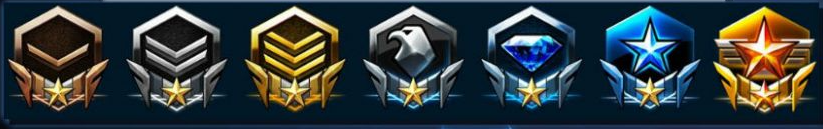
\includegraphics[scale=0.74]{../figures/ranks starcraft II.PNG} 

